%%%%%%%%%%%%%%%%%%%%%%%%%%%%%%%%%%%%%%%%%
% Beamer Presentation
% LaTeX Template
% Version 2.0 (March 8, 2022)
%
% This template originates from:
% https://www.LaTeXTemplates.com
%
% Author:
% Vel (vel@latextemplates.com)
%
% License:
% CC BY-NC-SA 4.0 (https://creativecommons.org/licenses/by-nc-sa/4.0/)
%
%%%%%%%%%%%%%%%%%%%%%%%%%%%%%%%%%%%%%%%%%

%----------------------------------------------------------------------------------------
%	PACKAGES AND OTHER DOCUMENT CONFIGURATIONS
%----------------------------------------------------------------------------------------

\documentclass[
	11pt, % Set the default font size, options include: 8pt, 9pt, 10pt, 11pt, 12pt, 14pt, 17pt, 20pt
	%t, % Uncomment to vertically align all slide content to the top of the slide, rather than the default centered
	%aspectratio=169, % Uncomment to set the aspect ratio to a 16:9 ratio which matches the aspect ratio of 1080p and 4K screens and projectors
]{beamer}

\graphicspath{{Images/}{./}} % Specifies where to look for included images (trailing slash required)

\usepackage{booktabs} % Allows the use of \toprule, \midrule and \bottomrule for better rules in tables

%----------------------------------------------------------------------------------------
%	SELECT LAYOUT THEME
%----------------------------------------------------------------------------------------

% Beamer comes with a number of default layout themes which change the colors and layouts of slides. Below is a list of all themes available, uncomment each in turn to see what they look like.

%\usetheme{default}
%\usetheme{AnnArbor}
%\usetheme{Antibes}
%\usetheme{Bergen}
%\usetheme{Berkeley}
%\usetheme{Berlin}
\usetheme{Boadilla} %me gusta
%\usetheme{CambridgeUS}
%\usetheme{Copenhagen}
%\usetheme{Darmstadt}
%\usetheme{Dresden}
%\usetheme{Frankfurt}
%\usetheme{Goettingen} %dos dos
%\usetheme{Hannover} %dos dos
%\usetheme{Ilmenau}
%\usetheme{JuanLesPins}
%\usetheme{Luebeck}
%\usetheme{Madrid}
%\usetheme{Malmoe}
%\usetheme{Marburg}
%\usetheme{Montpellier}
%\usetheme{PaloAlto}
%\usetheme{Pittsburgh}
%\usetheme{Rochester} %muy flat
%\usetheme{Singapore}
%\usetheme{Szeged}
%\usetheme{Warsaw}

%----------------------------------------------------------------------------------------
%	SELECT COLOR THEME
%----------------------------------------------------------------------------------------

% Beamer comes with a number of color themes that can be applied to any layout theme to change its colors. Uncomment each of these in turn to see how they change the colors of your selected layout theme.

%\usecolortheme{albatross}
%\usecolortheme{beaver}
%\usecolortheme{beetle}
%\usecolortheme{crane}
%\usecolortheme{dolphin}
%\usecolortheme{dove}
%\usecolortheme{fly}
%\usecolortheme{lily} %default
%\usecolortheme{monarca}
%\usecolortheme{seagull}
%\usecolortheme{seahorse}
%\usecolortheme{spruce}
%\usecolortheme{whale}
%\usecolortheme{wolverine}

%----------------------------------------------------------------------------------------
%	SELECT FONT THEME & FONTS
%----------------------------------------------------------------------------------------

% Beamer comes with several font themes to easily change the fonts used in various parts of the presentation. Review the comments beside each one to decide if you would like to use it. Note that additional options can be specified for several of these font themes, consult the beamer documentation for more information.

\usefonttheme{default} % Typeset using the default sans serif font
%\usefonttheme{serif} % Typeset using the default serif font (make sure a sans font isn't being set as the default font if you use this option!)
%\usefonttheme{structurebold} % Typeset important structure text (titles, headlines, footlines, sidebar, etc) in bold
%\usefonttheme{structureitalicserif} % Typeset important structure text (titles, headlines, footlines, sidebar, etc) in italic serif
%\usefonttheme{structuresmallcapsserif} % Typeset important structure text (titles, headlines, footlines, sidebar, etc) in small caps serif

%------------------------------------------------

%\usepackage{mathptmx} % Use the Times font for serif text
\usepackage{palatino} % Use the Palatino font for serif text

\usepackage[ruled,vlined]{algorithm2e}
%\usepackage{helvet} % Use the Helvetica font for sans serif text
\usepackage[default]{opensans} % Use the Open Sans font for sans serif text
\usepackage[spanish]{babel}
\usepackage{dirtree}
\usepackage{xcolor}
%\usepackage[default]{FiraSans} % Use the Fira Sans font for sans serif text
%\usepackage[default]{lato} % Use the Lato font for sans serif text

%----------------------------------------------------------------------------------------
%	SELECT INNER THEME
%----------------------------------------------------------------------------------------

% Inner themes change the styling of internal slide elements, for example: bullet points, blocks, bibliography entries, title pages, theorems, etc. Uncomment each theme in turn to see what changes it makes to your presentation.

%\useinnertheme{default}
\useinnertheme{circles}
%\useinnertheme{rectangles}
%\useinnertheme{rounded}
%\useinnertheme{inmargin}

%----------------------------------------------------------------------------------------
%	SELECT OUTER THEME
%----------------------------------------------------------------------------------------

% Outer themes change the overall layout of slides, such as: header and footer lines, sidebars and slide titles. Uncomment each theme in turn to see what changes it makes to your presentation.

%\useoutertheme{default}
%\useoutertheme{infolines}
%\useoutertheme{miniframes}
%\useoutertheme{smoothbars}
%\useoutertheme{sidebar}
%\useoutertheme{split}
%\useoutertheme{shadow}
%\useoutertheme{tree}
%\useoutertheme{smoothtree}

%\setbeamertemplate{footline} % Uncomment this line to remove the footer line in all slides
%\setbeamertemplate{footline}[page number] % Uncomment this line to replace the footer line in all slides with a simple slide count

%\setbeamertemplate{navigation symbols}{} % Uncomment this line to remove the navigation symbols from the bottom of all slides

%----------------------------------------------------------------------------------------
%	PRESENTATION INFORMATION
%----------------------------------------------------------------------------------------

\title[SEMINARIO DE INVESTIGACIÓN I]{Estrategias para la exploración coordinada multi-VANT} % The short title in the optional parameter appears at the bottom of every slide, the full title in the main parameter is only on the title page

%\subtitle{Optional Subtitle} % Presentation subtitle, remove this command if a subtitle isn't required

\author[Luis Ballado]{Luis Ballado} % Presenter name(s), the optional parameter can contain a shortened version to appear on the bottom of every slide, while the main parameter will appear on the title slide

\institute[CINVESTAV]{CINVESTAV - UNIDAD TAMAULIPAS \\ \smallskip \textit{luis.ballado@cinvestav.mx}} % Your institution, the optional parameter can be used for the institution shorthand and will appear on the bottom of every slide after author names, while the required parameter is used on the title slide and can include your email address or additional information on separate lines

\date[\today]{\today} % Presentation date or conference/meeting name, the optional parameter can contain a shortened version to appear on the bottom of every slide, while the required parameter value is output to the title slide

%----------------------------------------------------------------------------------------

\begin{document}

%----------------------------------------------------------------------------------------
%	TITLE SLIDE
%----------------------------------------------------------------------------------------

\begin{frame}
  \titlepage % Output the title slide, automatically created using the text entered in the PRESENTATION INFORMATION block above
\end{frame}

%----------------------------------------------------------------------------------------
%	TABLE OF CONTENTS SLIDE
%----------------------------------------------------------------------------------------

% The table of contents outputs the sections and subsections that appear in your presentation, specified with the standard \section and \subsection commands. You may either display all sections and subsections on one slide with \tableofcontents, or display each section at a time on subsequent slides with \tableofcontents[pausesections]. The latter is useful if you want to step through each section and mention what you will discuss.
\AtBeginSection[]
{
  \begin{frame}
    \frametitle{Contenido} % Slide title, remove this command for no title
    \tableofcontents[currentsection] % Output the table of contents (all sections on one slide)
    %\tableofcontents[pausesections] % Output the table of contents (break sections up across separate slides)
  \end{frame}
}
%----------------------------------------------------------------------------------------
%	PRESENTATION BODY SLIDES
%----------------------------------------------------------------------------------------

%\section{Introducción} % Sections are added in order to organize your presentation into discrete blocks, all sections and subsections are automatically output to the table of contents as an overview of the talk but NOT output in the presentation as separate slides

%------------------------------------------------

% Ejemplo imagen
%\begin{figure}
%  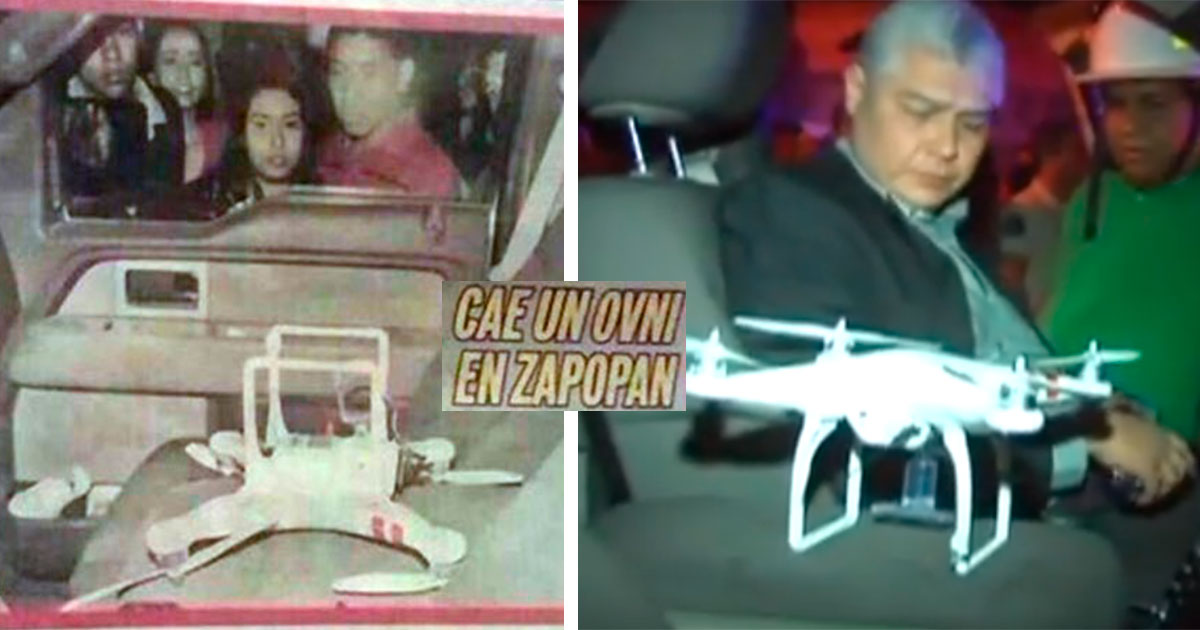
\includegraphics[width=0.7\linewidth]{dron_ovni.jpg}
%\end{figure}

\section{Resumen}

\begin{frame}
  
  \begin{block}{Resumen}

    {\footnotesize Las últimas decadas se ha visto una explosión en el interés de los Vehículos Aéreos No Tripulados (VANTs o drones), a la par que se han introducido nuevas tecnologías de comunicaciones y cómputo en la nube. Los avances en comunicación han permeado al control de VANTs logrando crear soluciones en búsqueda y rescate, así como soluciones de entrega en la última milla. La mayoria de estas aplicaciones carecen de ser autónomas. Para lograr la autonomía primero se deben resolver problemas clásicos en robótica móvil (Mapeo, Localización y Navegación).\\
      
    Se ha demostrado que es posible dotar de autonomía a un VANT y la mayoría de las soluciones son en exteriores con una mejor lectura de un sensor GPS. Los drones del mañana deberán navegar en áreas urbanas de la mejor manera posible y tener la habilidad de trabajar en coordinación con múltiples agentes.\\
    
    El enfoque de este trabajo es la creación y propuesta de una arquitectura capaz de coordinar múltiples-VANTs.\\
    }
  \medskip 
  
  \noindent \textbf{Palabras claves:} multi-VANT, coordinación multi-agente, arquitectura multi-VANT, 3D Path finding
  
  \end{block}
  
\end{frame}

\section{Descripción del proyecto}

\begin{frame}
  \frametitle{Descripción del proyecto}

  {\footnotesize
  El proyecto de estrategias para la exploración coordinada múlti-VANT se centra en las ventajas de tener múltiples-VANT(s) trabajando en conjunto para mejorar la eficiencia y cobertura de la exploración proponiendo una arquitectura de software que con ayuda de algoritmos que permitan la coordinación eficiente de múltiples-VANT(s) para llevar a cabo tareas de exploración en entornos desconocidos y cambiantes.}
      
\end{frame}

\begin{frame}

  \frametitle{Antecedentes y motivación para el proyecto}
  {\footnotesize
  Millones de Vehículos Aéreos No Tripulados, o también conocidos como drones, han presentado una adopción masiva en diferentes aplicaciones, desde usos civiles (búsqueda y rescate, monitoreo industrial, vigilancia), hasta aplicaciones militares [1]. La popularidad de los VANTs es atribuida a su movilidad omnidireccional.\\

  La idea de utilizar múltiples robots aéreos en un sistema coordinado se basa en el comportamiento de los enjambres de animales (como las abejas o los pájaros, que trabajan juntos de manera colaborativa para lograr objetivos comunes). Ésta inspiración biológica ha llevado al desarrollo de algoritmos y técnicas para coordinar y controlar múltiples VANTs en diferentes aplicaciones.\\

  El interés en la investigación e inovación de soluciones con Vehículos Aéreos No Tripulados ha crecido exponencialmente en años recientes [2,7,8,9,10].\\
  }
  \bigskip % Vertical whitespace
  {\footnotesize
  En recientes años, dotar a los VANTs de inteligencia para explotar la información recolectada de sensores a bordo ha sido y es un área de estudio en robótica móvil aérea (construcción de mapas)[3]. Así también los VANTs han sido un módelo interesante de estudio en control por ser marginalmente estable. Convirtiéndo los problemas típicos de control 2D (péndulo inverso fijo) a ambientes 3D [4].
  }
  
\end{frame}

\begin{frame}
  Calcular la ruta más corta entre dos puntos en un ambiente 3D es un problema NP-hard[21]. La mayoria de planificadores de rutas hacen uso de heuristicas y metaheuristicas para generar el óptimo más cercano \\
  \bigskip % Vertical whitespace
  Beneficios coordinación múlti-VANT
  \begin{itemize}
  \item Eficiencia y cobertura
  \item Redundancia y tolerancia a fallos
  \item Adaptabilidad a entornos dinámicos
  \item Distribución de carga de trabajo
  \item Aprendizaje colaborativo
  \end{itemize}
\end{frame}

\section{Planteamiento del problema}

\begin{frame}
  \frametitle{Planteamiento del problema}
  
  La coordinación múlti-VANT es un desafío complejo y plantea diversas problemáticas que deben abordarse.
  \bigskip % Vertical whitespace
  \begin{itemize}
  \item<1-> Coordinación - Establecer comunicación efectiva entre los múltiples VANTs. Intercambiar información relevante. Tener baja latencia en su comunicación.
  \item<2-> Planificación - Los VANTs deben coordinar sus movimientos para evitar colisiones y lograr una cobertura eficiente del área objetivo.
  \item<3-> Asignación de tareas - Se busca evitar la duplicación de esfuerzos optimizando el uso de recursos disponibles.
  \end{itemize}
  
\end{frame}

\begin{frame}
  Dada un área de interés \textbf{A} desconocido que se desea explorar, un conjunto de VANTs denotados como \textbf{$V=V_{1},V_{2},V_{3},...,V_{n}$}, donde $n$ es el número total de VANTs disponibles, un conjunto de tareas de exploración denotados como \textbf{$T=T_{1},T_{2},T_{3},...,T_{m}$}, donde $m$ es el número total de tareas a realizar.\\
  \bigskip % Vertical whitespace
  Teniendo restricciones y requisitos específicos del problema, como límites de tiempo, obstáculos a evitar ... etc.\\

  Para las tareas de exploración $T_{m}$, se considerán las siguientes variables:

  \begin{itemize}
  \item Posición inicial: $p_{i}(x,y,z)$, posición inical VANTs
  \item Trayectoria: $\alpha_{i}$, trayectoria seguida por los VANTs asignados a la tarea $T_{m}$ en función del tiempo t
  \item Información recolectada: $C_{i}$, representa la información recolectada por los VANTs asignados durante la exploración
  \end{itemize}
  
\end{frame}

\begin{frame}
  La función objetivo puede cambiar, algunos ejemplos pueden ser:
  \bigskip % Vertical whitespace
  \begin{itemize}
  \item Maximizar la cobertura del área de interés \textbf{A}
  \item Minimizar el tiempo total requerido para cubrir el área de interés \textbf{A}
  \item Maximizar la cantidad de información recolectada
  \end{itemize}
  
\end{frame}

\section{Objetivos generales y específicos del proyecto}

\begin{frame}
  
  \frametitle{Objetivos generales y específicos del proyecto}

  \begin{enumerate}
  \item<1-> General \\

    Desarrollo e implementación de una arquitectura de software tolerante a fallas para la coordinación de múltiples VANTs con un enfoque simulado en búsqueda y rescate.
        
  \item<2-> Particulares\\

    \begin{itemize}
    \item<1-> Generación del modelo dinámico de un VANT 
    \item<2-> Creación de algoritmos reactivos de baja memoria que garanticen evitar colisiones
    \item<3-> Eficiencia y rendimiento del sistema
    \item<4-> Adaptabilidad y flexibilidad, la coordinación múlti-VANT debe ser adaptable a cambios en el entorno, nuevos objetivos y adaptable a la incorporación o salida de VANTs durante la exploración
    \end{itemize}
    
  \end{enumerate}
\end{frame}

\section{Metodología}

\begin{frame}

  \frametitle{Metodología}
  \bigskip % Vertical whitespace

  \begin{enumerate}
  \item <1-> Revisión de literatura 
    \begin{itemize}
    \item Realizar una revisión de la literatura científica y técnica relacionada con la coordinación de múltiples VANTs
    \item Identificar los enfoques existentes, algoritmos y tecnologías usadas en la coordinación de múltiples VANTs
    \end{itemize}
  \item <2-> Análisis y diseño de la solución propuesta
    \begin{itemize}
    \item Identificar los requisitos clave para una coordinación eficiente
    \item Propuesta de algoritmos y políticas de navegación que permitan la coordinación eficiente
    \item Estrategias para la repartición de tareas y gestión de recursos.
    \end{itemize}
  \item <3-> Implementación y validación
    \begin{itemize}
    \item Hacer uso de simuladores (Son baratos, rápidos .. pero la solución está lejos de la solución propuesta en el ambiente real).
    \item Evaluar el desempeño de la coordinación
    \end{itemize}
  \item <4-> Evaluación, resultados y conclusiones
    \begin{itemize}
    \item Analizar y comparar los resultados obtenidos con otros enfoques existentes.
    \item Identificar posibles mejoras y áreas de investigación futuras
    \end{itemize}
  \end{enumerate}
  
\end{frame}


\section{Estado del Arte}

\begin{frame}

  %\frametitle{Estado del Arte}
  {\color{blue} Estado del Arte}
  \dirtree{%
    .1 Robótica Móvil.
    .2 Robótica Móvil Terrestre.
    .2 Robótica Móvil Aérea.
    .3 Dinámica de un Vehículo Aéreo No Tripulado.
    .3 Control de un Vehículo Aéreo No Tripulado.
    .2 Problemas en la Robótica Móvil.
    .3 Mapas.
    .4 Construcción y representación de mapas 3D.
    .5 Percepción.
    .6 Sensores LiDAR.
    .6 Sensores Cámaras (Odometría Visual).
    .3 Localización.
    .3 Planificación de trayectorias.
    .2 Robótica Colaborativa (múltiples robots).
    .3 Exploración.
    .3 Coordinación.
    .3 Colaboración.
    .2 Arquitectura de Software en robótica.
  }
\end{frame}

\begin{frame}

  La \textbf{robótica móvil} ha experimentado avances significativos en los últimos años, transformando múltiples sectores y abriendo nuevas posibilidades en la automatización.\\
  Los robots móviles se pueden ver como sistemas autónomos capaces de moverse y operar en entornos cambiantes y complejos sin la necesidad de guías físicas.\\
  
\bigskip % Vertical whitespace

En cuanto a la navegación, se han desarrollado técnicas de localización y mapeo simultáneos (SLAM) más precisas y eficientes, permitiendo construir mapas detallados de su entorno y ubicarse con mayor precisión en tiempo real. Además, se han mejorado los algoritmos de planificación de trayectorias para garantizar movimientos seguros y eficientes en entornos dinámicos.\\
\end{frame}
\begin{frame}
Robótica Móvil
\begin{itemize}
\item <1-> Robótica Móvil Terrestre (con ruedas)\\
  \begin{itemize}
  \item Ackerman
  \item Triciclo clásico
  \item Omnidireccionales
  \item Diferenciales
  \end{itemize}
\item <2-> Robótica Móvil Aérea\\
  \begin{itemize}
  \item Ala fija
  \item Rotores
    \begin{itemize}
    \item Rotor único
    \item Multi-rotor
    \end{itemize}
  \end{itemize}
  \item <3-> Hibridos VTOL
\end{itemize}
\end{frame}

\begin{frame}
  \begin{figure}
    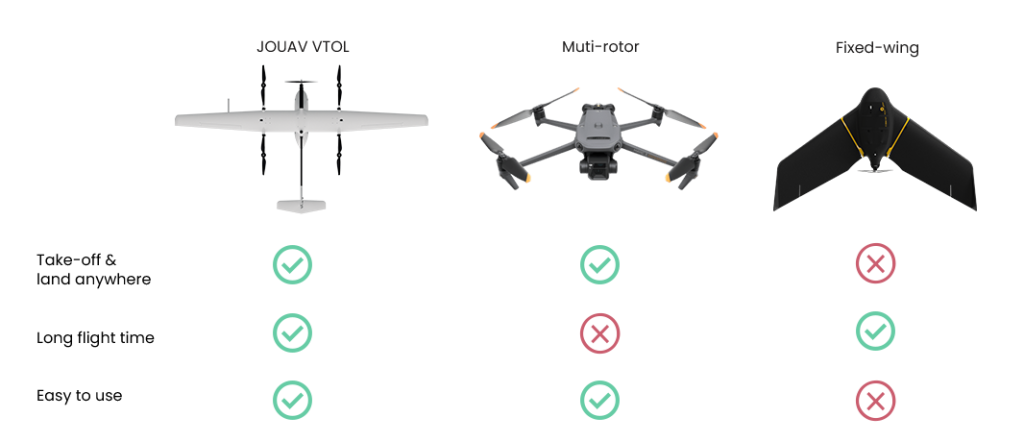
\includegraphics[width=0.9\linewidth]{drones.png}
  \end{figure}
\end{frame}

\begin{frame}
  \textbf{Dinámica de un Vehículo Aéreo No Tripulado}

  \begin{figure}
    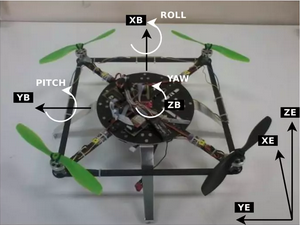
\includegraphics[width=0.5\linewidth]{d4.png}
  \end{figure}

  \begin{figure}
    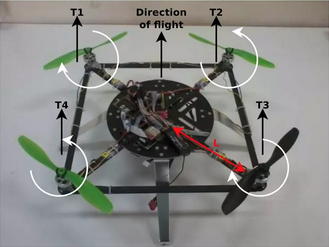
\includegraphics[width=0.5\linewidth]{d5.png}
  \end{figure}
\end{frame}

\begin{frame}
  Problemas en la Robótica móvil
  \begin{itemize}
  \item Mapas
  \item Localización
  \item Planificación de trayectorias
  \end{itemize}
\end{frame}


\begin{frame}
  Construcción y representación de mapas 3D\\
  Percepción
  \begin{itemize}
  \item Sensores LiDAR
  \item Sensores Cámaras (Odometría Visual)
  \end{itemize}
\end{frame}

%\begin{frame}
%  Localización 
%\end{frame}

\begin{frame}
  \textbf{Planificación de trayectorias}\\
         {\footnotesize
  Dentro de la literatura a esta problemática se encuentran estudios que minimizan el tiempo de vuelo [16], la altitud de vuelo [17], y la velocidad del dron [18]. Podemos categorizar los panificadores de trayectoria dos grupos \textbf{offline y online}\\
  Los planificadores Online dado que utilizan sensores y reaccionan a obstáculos no garantizan en dar el camino más óptimo.\\

  Apesar que existen múltiples estudios donde reducen el problema de 3D a 2D [19,20]. Limitando la movilidad del VANT haciendo que los algoritmos propuestos para robótica móvil terrestre puedan ser aplicados directamente. 
  }
  \begin{figure}
    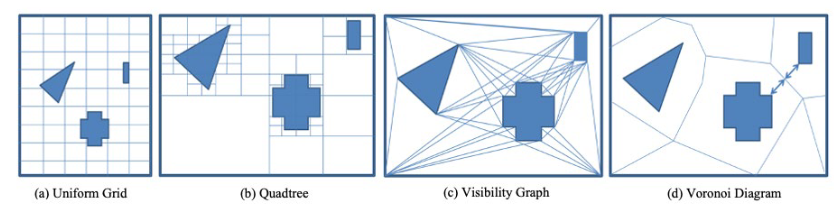
\includegraphics[width=0.8\linewidth]{maps.png}
    \caption{Representación del medio ambiente}
  \end{figure}
  
\end{frame}

%\begin{frame}
%  Robótica Colaborativa

%  \begin{itemize}
%  \item Exploración
%  \item Coordinación
%  \item Colaboración
%  \end{itemize}
  
%\end{frame}

%\begin{frame}
%  Arquitectura de software en robótica
%\end{frame}

\section{Contribuciones o resultados esperados}

\begin{frame}

  \frametitle{Contribuciones o resultados esperados}

  \begin{enumerate}
  \item<1-> Códigos a disposición de la comunidad
  \item<2-> Simulación de solución
  \item<3-> Tesis impresa
  \end{enumerate}
  
\end{frame}

\end{document} 
